% Fig. 1 -- baseline migration protocol, TikZ port of figs/1.pdf.
% Coordinates are the original artwork's PostScript points (bp), measured
% from its top-left corner (y grows downwards), so the picture is exactly
% 165.088bp x 133.709bp like the PDF. Museo Sans / Myriad Pro are replaced
% by Helvetica, with each label stretched to the original label's width.
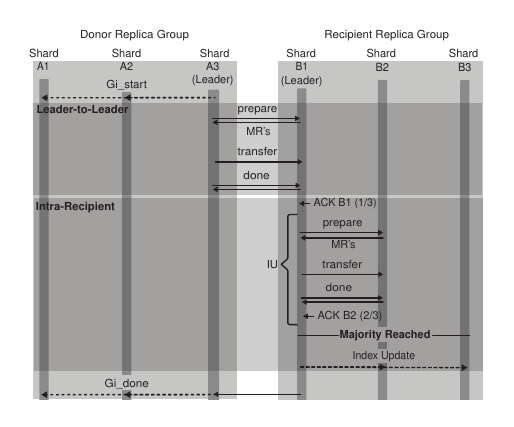
\begin{tikzpicture}[x=1bp,y=-1bp,
    lbl/.style={inner sep=0pt,outer sep=0pt,anchor=base west,text=ink,
                font=\fontsize{4bp}{4.8bp}\fontfamily{phv}\selectfont},
    bold/.append style={font=\fontsize{4bp}{4.8bp}\fontfamily{phv}\bfseries},
    msg/.style={draw=ink,line width=0.5bp,line cap=round,line join=round},
    gi/.style={draw=ink,line width=0.5bp},
    iu/.style={msg,dash pattern=on 1bp off 1bp},
    head/.style={fill=ink},
    lifeline/.style={fill=lifegray,rounded corners=0.283bp},
    band/.style={fill=ink,fill opacity=0.22},
  ]
  \definecolor{ink}{RGB}{35,31,32}
  \definecolor{groupbg}{RGB}{198,198,197}
  \definecolor{lifegray}{RGB}{140,139,140}
  \useasboundingbox (0,0) rectangle (165.088,133.709);
  \clip (0,0) rectangle (165.088,133.709);

  % replica-group backgrounds
  \fill[groupbg] (1.835,11.938) rectangle (75.535,133.709); % donor
  \fill[groupbg] (90.132,11.939) rectangle (163.833,175.872); % recipient

  % shard lifelines (they run past the bottom edge, as in the original)
  \fill[lifeline] (4.221,18.405) rectangle (7.554,175.872); % A1
  \fill[lifeline] (33.959,18.303) rectangle (37.292,175.72); % A2
  \fill[lifeline] (64.977,22.331) rectangle (68.916,175.872); % A3
  \fill[lifeline] (96.984,21.867) rectangle (100.317,176.355); % B1
  \fill[lifeline] (126.03,18.814) rectangle (129.363,175.998); % B2
  \fill[lifeline] (155.689,18.864) rectangle (159.022,176.498); % B3

  % headers
  \node[lbl] at (0.551,10.749) {\scalebox{0.994}[1.019]{Shard}};
  \node[lbl] at (3.441,15.516) {\scalebox{0.913}[1.019]{A1}};
  \node[lbl] at (30.289,10.731) {\scalebox{0.994}[1.019]{Shard}};
  \node[lbl] at (33.18,15.394) {\scalebox{0.981}[0.989]{A2}};
  \node[lbl] at (62.03,10.679) {\scalebox{0.994}[1.003]{Shard}};
  \node[lbl] at (64.254,15.368) {\scalebox{0.977}[1.003]{A3}};
  \node[lbl] at (59.15,20.183) {\scalebox{0.992}[1.003]{(Leader)}};
  \node[lbl] at (93.169,10.717) {\scalebox{0.994}[1]{Shard}};
  \node[lbl] at (96.427,15.518) {\scalebox{0.918}[1]{B1}};
  \node[lbl] at (91.179,20.318) {\scalebox{0.992}[1]{(Leader)}};
  \node[lbl] at (121.994,10.726) {\scalebox{0.994}[1.017]{Shard}};
  \node[lbl] at (125.273,15.611) {\scalebox{0.986}[1.017]{B2}};
  \node[lbl] at (151.651,10.753) {\scalebox{0.994}[1.020]{Shard}};
  \node[lbl] at (154.931,15.651) {\scalebox{0.982}[1.020]{B3}};
  \node[lbl] at (18.843,3.798) {\scalebox{1.045}[1]{Donor Replica Group}};
  \node[lbl] at (106.827,4.014) {\scalebox{1.034}[1]{Recipient Replica Group}};

  % "Majority Reached" rule
  \draw[msg] (97.43,110.781) -- (111.831,110.781);
  \draw[msg] (145.81,110.92) -- (159.088,110.92);
  \fill[groupbg] (112.35,107.918) rectangle (144.83,113.194); % Majority Reached
  \node[lbl,bold] at (112.331,112.001) {\scalebox{0.988}[1]{Majority Reached}};

  % intra-recipient: B1 <-> B2, and the IU brace
  \node[lbl] at (104.359,105.037) {\scalebox{0.996}[1]{ACK B2 (2/3)}};
  \draw[msg] (102.942,103.9) -- (100.582,103.9);
  \fill[head] (100.874,102.902) -- (99.147,103.899) -- (100.874,104.897) -- cycle;
  \draw[msg] (98.521,97.275) -- (126.457,97.275);
  \fill[head] (126.165,98.272) -- (127.892,97.275) -- (126.165,96.277) -- cycle;
  \draw[msg] (127.892,98.8) -- (100.137,98.8);
  \fill[head] (100.429,97.803) -- (98.702,98.8) -- (100.429,99.798) -- cycle;
  \node[lbl] at (107.298,95.019) {\scalebox{1.072}[1]{done}};
  \draw[msg] (98.757,88.783) -- (126.551,88.783);
  \fill[head] (126.259,89.78) -- (127.986,88.783) -- (126.259,87.785) -- cycle;
  \node[lbl] at (106.127,86.525) {\scalebox{1.068}[1]{transfer}};
  \draw[msg] (97.008,67.238) -- (94.261,67.238) .. controls (93.948,67.238) and (93.694,67.461) .. (93.694,67.736)
    -- (93.694,82.696) .. controls (93.694,82.955) and (93.577,83.203) .. (93.369,83.386)
    -- (91.393,85.12) -- (91.302,85.201) -- (93.369,87.016) .. controls (93.577,87.198) and (93.694,87.446) .. (93.694,87.705)
    -- (93.694,106.425) .. controls (93.694,106.7) and (93.948,106.923) .. (94.261,106.923) -- (97.008,106.923); % IU brace
  \node[lbl] at (86.068,86.765) {\scalebox{1.019}[1]{IU}};
  \draw[msg] (98.043,73.779) -- (126.495,73.779);
  \fill[head] (126.202,74.776) -- (127.929,73.779) -- (126.202,72.781) -- cycle;
  \draw[msg] (127.929,75.689) -- (99.659,75.689);
  \fill[head] (99.951,74.692) -- (98.224,75.689) -- (99.951,76.687) -- cycle;
  \node[lbl] at (109.315,79.451) {\scalebox{0.976}[1]{MR's}};
  \node[lbl] at (106.243,71.523) {\scalebox{1.039}[1]{prepare}};
  \node[lbl] at (102.967,64.447) {\scalebox{0.968}[1]{ACK B1 (1/3)}};
  \draw[msg] (101.552,63.312) -- (99.191,63.312);
  \fill[head] (99.483,62.315) -- (97.756,63.312) -- (99.483,64.31) -- cycle;

  % leader-to-leader: A3 <-> B1
  \draw[msg] (66.674,56.795) -- (96.725,56.795);
  \fill[head] (96.433,57.792) -- (98.16,56.795) -- (96.433,55.797) -- cycle;
  \draw[msg] (98.16,58.212) -- (68.109,58.212);
  \fill[head] (68.401,57.215) -- (66.674,58.212) -- (68.401,59.21) -- cycle;
  \node[lbl] at (77.654,54.537) {\scalebox{1.072}[1]{done}};
  \draw[msg] (67.627,48.303) -- (97.545,48.303);
  \fill[head] (97.253,49.3) -- (98.98,48.303) -- (97.253,47.305) -- cycle;
  \node[lbl] at (75.594,45.987) {\scalebox{1.068}[1]{transfer}};
  \draw[msg] (66.526,32.678) -- (96.577,32.678);
  \fill[head] (96.286,33.675) -- (98.013,32.678) -- (96.286,31.68) -- cycle;
  \draw[msg] (98.013,34.095) -- (67.962,34.095);
  \fill[head] (68.253,33.098) -- (66.526,34.095) -- (68.253,35.093) -- cycle;
  \node[lbl] at (78.71,38.913) {\scalebox{0.976}[1]{MR's}};
  \node[lbl] at (75.574,30.421) {\scalebox{1.039}[1]{prepare}};

  % Gi_done: B1 -> A3 (solid), A3 -> A1/A2 (dashed)
  \draw[msg] (98.342,131.974) -- (68.291,131.974);
  \fill[head] (68.582,130.977) -- (66.856,131.974) -- (68.582,132.972) -- cycle;
  \draw[gi] (67.439,132.065) -- (66.939,132.066);
  \draw[gi,dash pattern=on 1.013bp off 1.013bp] (65.926,132.067) -- (7.68,132.132);
  \draw[gi] (7.173,132.133) -- (6.673,132.134);
  \fill[head] (7.037,130.886) -- (4.88,132.135) -- (7.04,133.379) -- cycle;
  \draw[gi] (65.452,132.093) -- (64.952,132.093);
  \draw[gi,dash pattern=on 1.031bp off 1.031bp] (63.921,132.094) -- (37.638,132.106);
  \draw[gi] (37.122,132.106) -- (36.622,132.106);
  \fill[head] (36.987,130.86) -- (34.829,132.108) -- (36.988,133.353) -- cycle;

  % Gi_start: A3 -> A1/A2 (dashed)
  \draw[gi] (67.534,25.177) -- (67.034,25.178);
  \draw[gi,dash pattern=on 1.013bp off 1.013bp] (66.022,25.179) -- (7.776,25.244);
  \draw[gi] (7.268,25.244) -- (6.768,25.245);
  \fill[head] (7.132,23.998) -- (4.975,25.247) -- (7.135,26.491) -- cycle;
  \draw[gi] (65.547,25.187) -- (65.047,25.187);
  \draw[gi,dash pattern=on 1.031bp off 1.031bp] (64.016,25.188) -- (37.733,25.2);
  \draw[gi] (37.218,25.2) -- (36.718,25.2);
  \fill[head] (37.082,23.954) -- (34.924,25.202) -- (37.083,26.447) -- cycle;

  % Index Update: B1 -> B2/B3 (dotted)
  \draw[iu] (98.296,122.19) -- (127.09,122.19);
  \fill[head] (126.725,123.436) -- (128.883,122.189) -- (126.725,120.944) -- cycle;
  \draw[iu] (98.296,122.19) -- (156.578,122.389);
  \fill[head] (156.209,123.634) -- (158.372,122.395) -- (156.218,121.141) -- cycle;

  % labels sitting on knock-outs of the group background
  \fill[groupbg] (21.506,17.334) rectangle (49.852,23.003); % Gi_start
  \node[lbl] at (28.335,21.904) {\scalebox{1.036}[1]{Gi{\fontencoding{T1}\selectfont\_}start}};
  \fill[groupbg] (21.517,124.917) rectangle (49.863,130.586); % Gi_done
  \node[lbl] at (27.715,129.487) {\scalebox{1.055}[1]{Gi{\fontencoding{T1}\selectfont\_}done}};
  \fill[groupbg] (114.028,115.74) rectangle (142.333,120.551); % Index Update
  \node[lbl] at (116.982,119.319) {\scalebox{0.951}[1]{Index Update}};

  % phase bands: 22% ink overlays drawn over everything, labels on top
  \fill[band] (2.068,27.101) rectangle (163.643,60.149); % Leader-to-Leader
  \node[lbl,bold] at (3.194,31.029) {\scalebox{1.016}[1]{Leader-to-Leader}};
  \fill[band] (2.297,61.204) rectangle (163.872,123.566); % Intra-Recipient
  \node[lbl,bold] at (2.961,65.754) {\scalebox{1.016}[1]{Intra-Recipient}};
\end{tikzpicture}%
